\documentclass{TIJMUjiaoanLL}
\pagestyle{empty}


\begin{document}


%课程名称
\kecheng{Linux系统概论}
%课程内容
\neirong{用户和组\ /\ 第3章}
%教师姓名
\jiaoshi{伊现富}
%职称
\zhicheng{讲师}
%教学日期(格式:XXXX年XX月XX日XX时-XX时)
\riqi{2015年5月19日13:30-15:20}
%授课对象(格式:XXX系XXXX年级XX班(硕/本/专科))
\duixiang{生物医学工程与技术学院2013级生信班(本)}
%听课人数
\renshu{28}
%授课方式
\fangshi{理论讲授}
%学时数
\xueshi{2}
%教材版本
\jiaocai{Unix入门经典,第1版}


%教案首页
\firstHeader
\maketitle
\thispagestyle{empty}

\mudi{
\begin{itemize}
  \item 掌握/etc/passwd文件的格式,Linux中“一切皆文件”的思想,账户管理的基本命令及命令的常用选项,进行身份变换的常用命令。
  \item 熟悉Linux中的三类账户,账户管理相关的配置文件、每个文件的作用以及它们之间的关系,/etc/shadow文件的格式,/etc/group文件的格式。
  \item 了解/etc/gshadow文件的格式,su和sudo的区别。
  \item 自学账户管理的辅助命令。
\end{itemize}
}

\fenpei{
\begin{itemize}
  \item (5')引言与导入:通过邮箱、网上商城、论坛等通行证/账号的例子引入账户的概念。
  \item (5')账户:介绍Linux中的三大类账户,讲解组账户的概念及权限管理中的三类用户。
  \item (40')用户管理文件:介绍账户管理相关的配置文件及其各自的作用,重点讲解/etc/passwd文件的格式,简单讲解其他配置文件的格式,总结配置文件之间的关系。
  \item (25')管理账户和组:分别介绍手动和命令管理账户的方式,传递“Linux一切皆文件”的思想,讲解账户管理的基本命令及其常用选项。
  \item (15')身份变换:介绍进行身份变换的su和sudo两个命令,并对两者进行比较。
  \item (5')辅助命令:简要介绍与账户管理相关的其他命令。
  \item (5')总结与答疑:总结授课内容中的知识点与技能,解答学生疑问。
\end{itemize}
}

\zhongdian{
\begin{itemize}
  \item 重点:/etc/passwd文件的格式,账户管理的基本命令及其常用选项。
  \item 难点:/etc/passwd文件的格式。
  \item 解决策略:通过实例讲解与操作演示帮助学生理解、记忆。
\end{itemize}
}

\waiyu{
  \vspace*{-10pt}
  \begin{multicols}{2}
    用户ID(User ID,UID)

    组ID(Group ID,GID)
  \end{multicols}
  \vspace*{-10pt}
}

\fuzhu{
\begin{itemize}
  \item 多媒体:账户管理相关的配置文件,文件格式,以及文件之间的关系。
  \item 板书:/etc/passwd文件的格式。
  \item 演示:账户管理的相关命令,命令操作对配置文件的影响。
\end{itemize}
}

\sikao{
  \vspace*{-10pt}
  \begin{multicols}{2}
  \begin{itemize}
    \item Linux系统中主要有哪三种类型的账户?
    \item 用户和组管理相关的文件主要有哪些?
    \item 解释/etc/passwd中各个字段的含义。
    \item 根据要求,使用useradd创建一个新账户。
    \item 改变用户身份的方法有哪些?
    \item 列举几个用户和组管理的辅助命令。
  \end{itemize}
  \end{multicols}
  \vspace*{-10pt}
}

\cankao{
\begin{itemize}
  %\item (美)Paul Love,Joe Merlino\ 等著,张楚雄,许文昭\ 译。Unix入门经典,清华大学出版社,2006。
  \item (美)Harley Hahn\ 著,张杰良\ 译。Unix \& Linux大学教程,清华大学出版社,2010。
  \item 鸟哥\ 著,王世江\ 改编。鸟哥的Linux私房菜——基础学习篇(第三版),人民邮电出版社,2010。
  \item 维基百科等网络资源。
\end{itemize}
}

\firstTail


%教案续页
\newpage
\otherHeader

\begin{enumerate}
  \item 引言与导入(5分钟)

    开门需要钥匙,论坛需要注册,邮箱需要登录……\textcolor{red}{有账户才有使用权!}

  \item 账户(5分钟)
    \begin{enumerate}
      \item 三类账户
	\begin{itemize}
	  \item 根账户/根用户/超级用户账户:Linux系统中的“上帝”
	  \item 系统账户:与软件或服务相关
\parpic[fr]{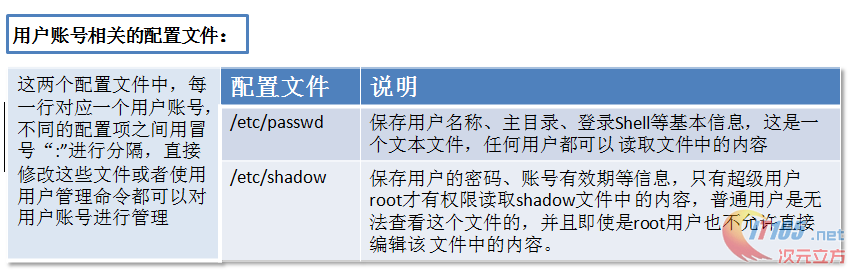
\includegraphics[width=9.3cm]{c2.user.file.png}}
	  \item 用户账户:普通用户账户
	\end{itemize}
      \item 组账户(群组)
	\begin{itemize}
	  \item 多个账户集中在一起形成一个组
	  \item 一个组可以包括多个账户
	  \item 一个账户至少属于一个组
	\end{itemize}
      \item 权限管理中的用户
	\begin{itemize}
\parpic[fr]{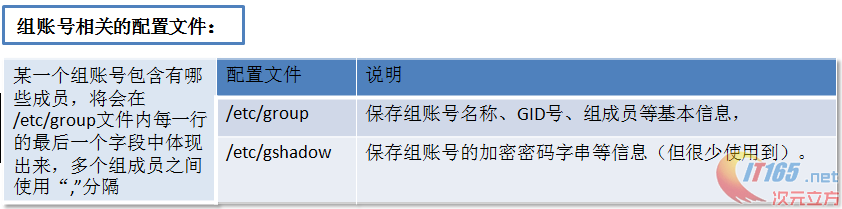
\includegraphics[width=9.3cm]{c2.group.file.png}}
	  \item 用户:文件的所有者
	  \item 组:指派给文件的组
	  \item 其他:系统中既不是所有者也不属于组的用户
	\end{itemize}
    \end{enumerate}

  \item 用户管理文件(40分钟)
    \begin{enumerate}
      \item 相关配置文件
	%\vspace*{-10pt}
        %\begin{table}[h]
          %\centering
          %\begin{tabularx}{0.62\textwidth}{cll}
            %\hline
            %文件 & 用途 & 说明\\
            %\hline
            %/etc/passwd & 为系统识别已授权的用户 & 用户账号相关\\
            %/etc/shadow & 保存相应账户加密后的口令 & 用户账号相关\\ 
	    %\hline
	    %/etc/group & 存放组账户的信息 & 组账号相关\\
	    %/etc/gshadow & 保存组账户加密后的口令 & 组账号相关\\
	    %\hline
          %\end{tabularx}
        %\end{table}
	\item \textcolor{red}{\textbf{【重点、难点】}}/etc/passwd\textcolor{red}{(通过实例解析辅助记忆)}
	\vspace*{-10pt}
	\begin{figure}[h]
	  \centering
	  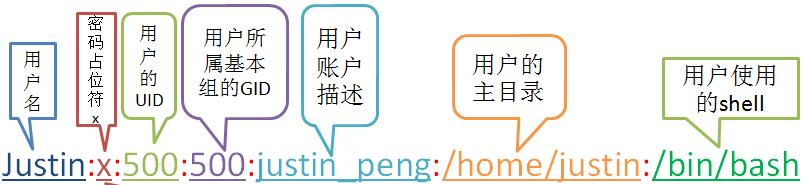
\includegraphics[width=14cm,height=3cm]{c2.passwd.fields.01.png}
	\end{figure}

      \item /etc/shadow
	\vspace*{-10pt}
	\begin{figure}[h]
	  \centering
	  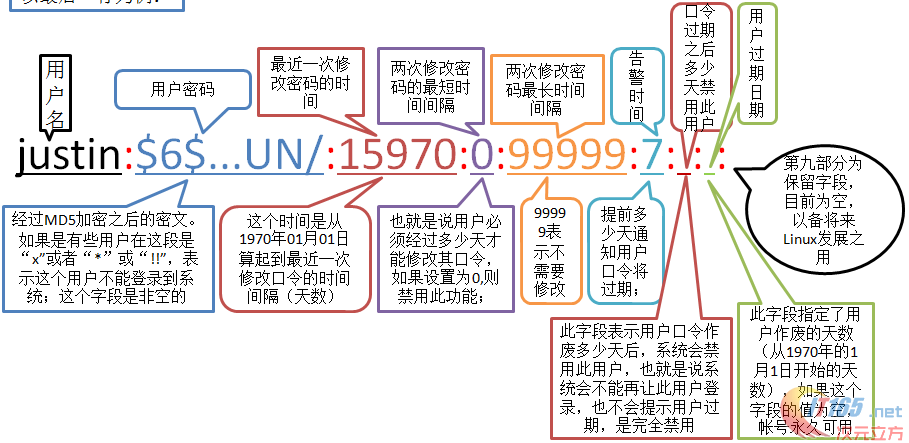
\includegraphics[width=14cm,height=6cm]{c2.shadow.fields.png}
	\end{figure}

	\vspace*{-25pt}
      \item /etc/group与/etc/gshadow
	\vspace*{-10pt}
	\begin{figure}[h]
	  \centering
	  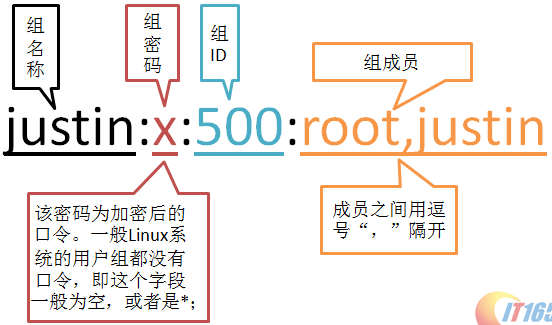
\includegraphics[width=7cm,height=4cm]{c2.group.fields.01.png}
	  \quad
	  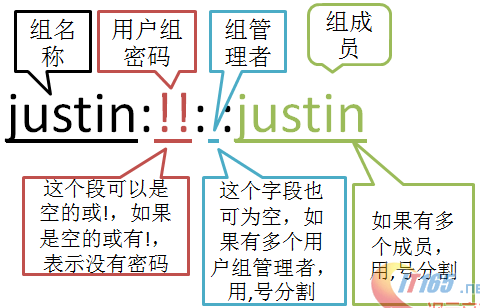
\includegraphics[width=7cm,height=4cm]{c2.gshadow.fields.png}
	\end{figure}

\otherTail
\newpage
\otherHeader

      \item 配置文件的关系
\parpic[fr]{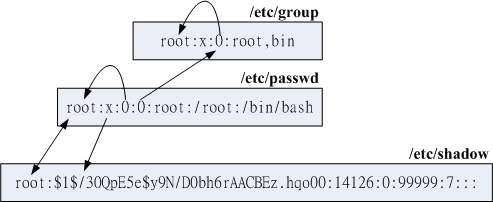
\includegraphics[width=8.2cm]{c2.etc.png}}
	%\begin{figure}[h]
	  %\centering
	  %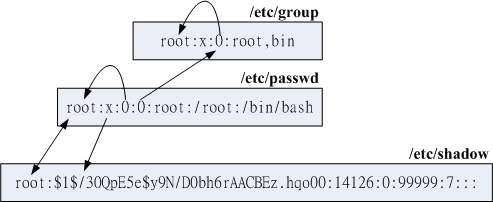
\includegraphics[width=12cm]{c2.etc.png}
	%\end{figure}
    \end{enumerate}

  \item 管理账户和组(25分钟)
    \begin{enumerate}
      \item 手动管理
	\begin{enumerate}
          \item 修改/etc/passwd:添加或删除账户行
          \item 修改/etc/shadow:添加或删除账户行
          \item 修改/etc/group:添加或删除账户引用
          \item 添加或删除账户的家目录
	\end{enumerate}
      \item 命令管理
	\begin{itemize}
\parpic[fr]{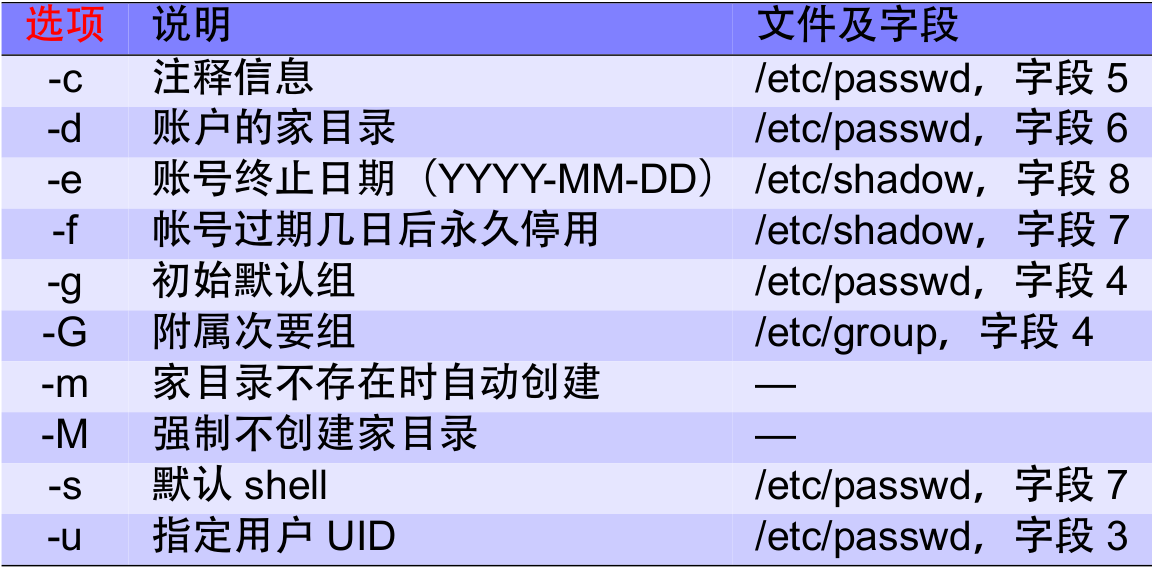
\includegraphics[width=8.5cm]{c2.useradd.options.png}}
	  \item 添加/修改/删除账户:useradd,usermod,userdel
	  \item 添加/修改/删除组:groupadd,groupmod,groupdel
	\end{itemize}
      \item 账户管理
	\begin{enumerate}
	  \item \textcolor{red}{\textbf{【重点】}}useradd的选项
	    \begin{itemize}
	      \item \textcolor{red}{进行实例的操作演示帮助记忆}
	      \item Linux系统中,“一切皆是文件”!
	      \item 命令操作的本质就是修改相应的配置文件。
	    \end{itemize}

	  \item 账户管理步骤
	    \begin{itemize}
	      \item 添加账户:useradd USERNAME
	      \item 创建密码:passwd USERNAME
	      \item 修改账户:usermod -l USERNAME.NEW USERNAME.OLD
	      \item 删除账户:userdel [-r] USERNAME,
	    \end{itemize}
	\end{enumerate}
      \item 组管理
	\begin{enumerate}
	  \item 组管理步骤
	    \begin{itemize}
	      \item 添加组:groupadd -g GID GROUPNAME
	      \item 修改组:groupmod -n GN.NEW GN.OLD
	      \item 删除组:groupdel GROUPNAME
	    \end{itemize}
	\end{enumerate}
    \end{enumerate}

  \item 身份变换(15分钟)
    \begin{enumerate}
\parpic[fr]{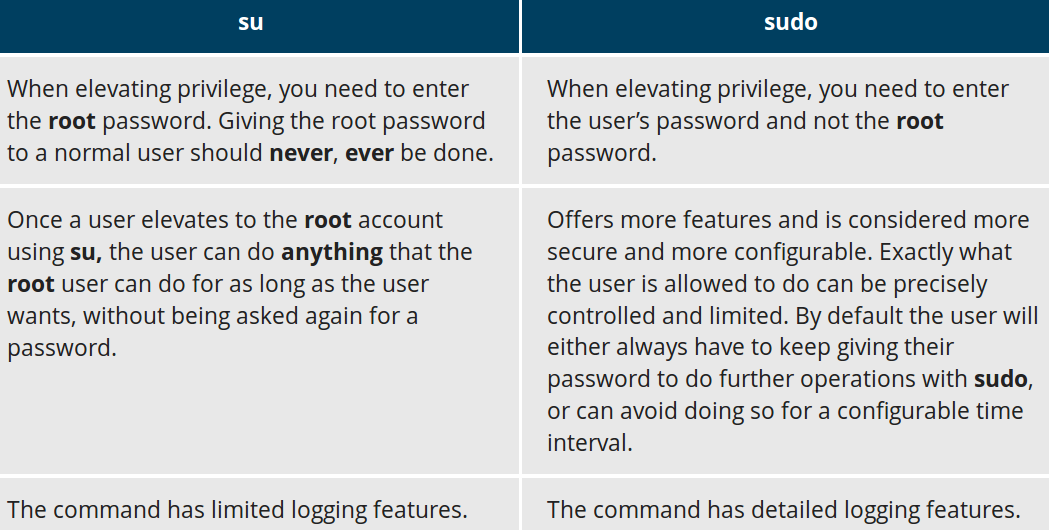
\includegraphics[width=8.5cm]{c2.su.sudo.png}}
      \item su:Switch User,su、su [-] USERNAME
      \item sudo:superuser do,sudo COMMAND
      \item su vs. sudo:sudo比su更安全
    \end{enumerate}

  \item 辅助命令(5分钟)\textcolor{red}{(通过操作演示进行讲解)}

    w,who,whoami, who am i,id,groups,finger,……

  \item 总结与答疑(5分钟)
    \begin{enumerate}
      \item 知识点
	\begin{itemize}
	  \item Linux系统中的三类账户
	  \item 账户管理的相关配置文件
	  \item 管理账户和组的常用命令
	  \item 变换用户身份的方法
	  \item 账户和组管理的辅助命令
	\end{itemize}
      \item 技能
	\begin{itemize}
	  \item 管理账户:创建、修改、删除
	  \item 管理组:创建、修改、删除
	\end{itemize}
    \end{enumerate}

\end{enumerate}

\otherTail


\end{document}

